\prefacesection{Appendix B: Reference Papers}
% Creates a section titled "Appendix B: Reference Papers" for displaying the reference papers.
%
%
% Paper 1
\vspace{-5mm}
% Adds vertical space of -5mm, reducing the space between the title and the first paper.
\textbf{[B1.]}
% Displays "B1." in bold to represent the first reference paper.
%
%
%
\begin{figure}[h!]
    \centering
    % Centers the figure on the page.
    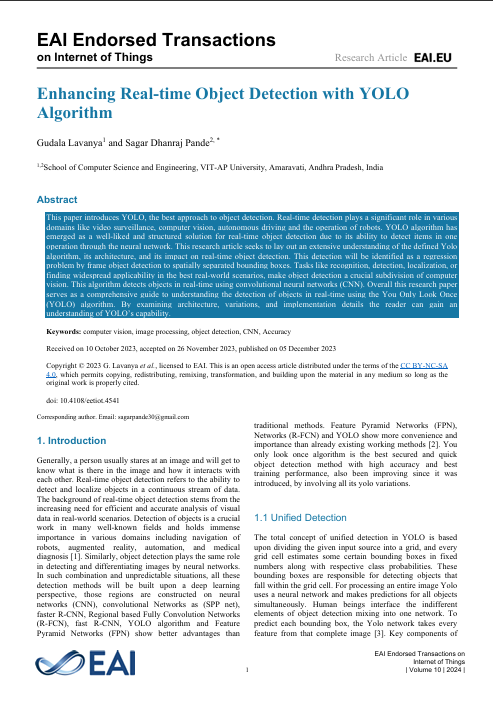
\includegraphics[width=0.8\textwidth]{reference_papers/Paper_1.png}
    % Includes an image of Paper 1 from the 'reference_papers' folder.
    % The image is scaled to 80% of the text width (0.8\textwidth).
\end{figure}
% Ends the figure environment for Paper 1.
%
%
% Paper 2
\\\\
% Inserts two line breaks before Paper 2.
\textbf{[B2.]}
% Displays "B2." in bold to represent the second reference paper.
%
%
%
\begin{figure}[h!]
    \centering
    % Centers the figure on the page.
    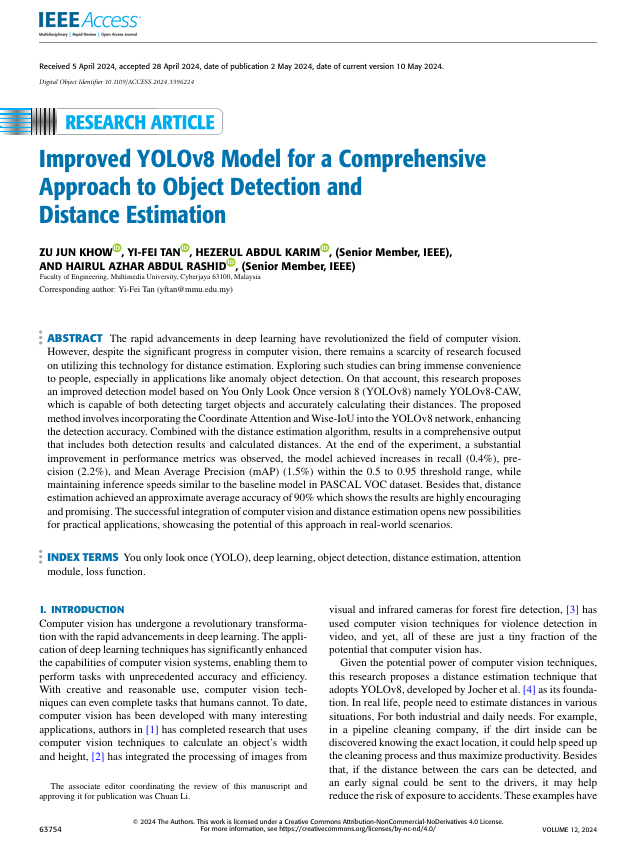
\includegraphics[width=1\textwidth]{reference_papers/Paper_2(Base Paper).png}
    % Includes an image of Paper 2 (Base Paper) from the 'reference_papers' folder.
    % The image is scaled to the full width of the text area (1\textwidth).
\end{figure}
% Ends the figure environment for Paper 2.
%
%
% Paper 3
\\\\\\\\
% Inserts four line breaks before Paper 3.
\textbf{[B3.]}
% Displays "B3." in bold to represent the third reference paper.
%
%
%
\begin{figure}[h!]
    \centering
    % Centers the figure on the page.
    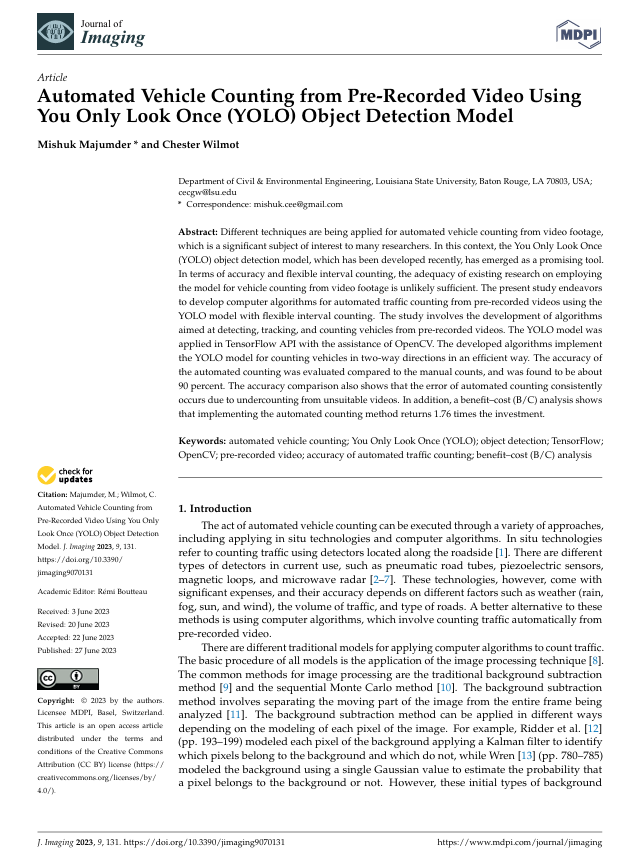
\includegraphics[width=1\textwidth]{reference_papers/Paper_3.png}
    % Includes an image of Paper 3 from the 'reference_papers' folder.
    % The image is scaled to the full width of the text area (1\textwidth).
\end{figure}
% Ends the figure environment for Paper 3.
%
%
% Paper 4
\\\\\\\\
% Inserts two line breaks before Paper 4.
\textbf{[B4.]}
% Displays "B4." in bold to represent the fourth reference paper.
%
%
%
\begin{figure}[h!]
    \centering
    % Centers the figure on the page.
    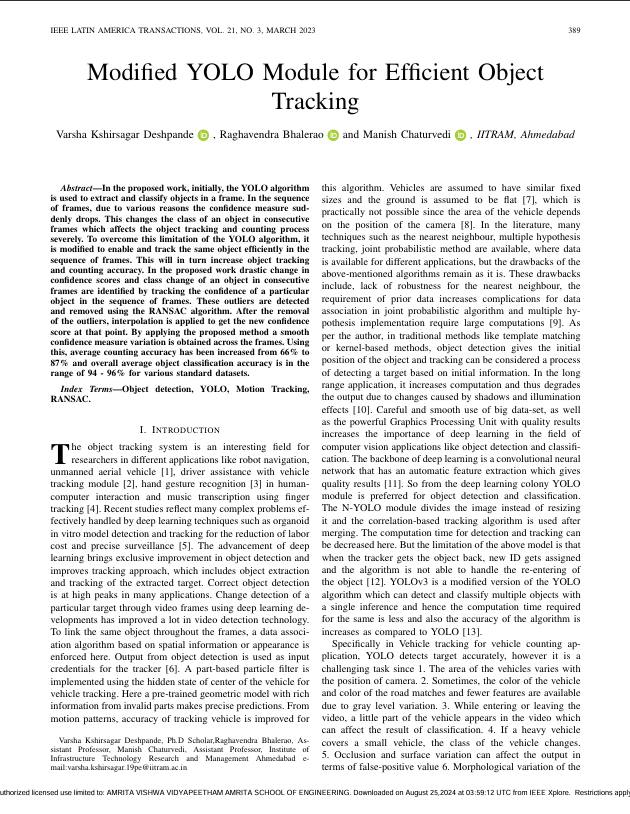
\includegraphics[width=1\textwidth]{reference_papers/Paper_4.png}
    % Includes an image of Paper 4 from the 'reference_papers' folder.
    % The image is scaled to the full width of the text area (1\textwidth).
\end{figure}
% Ends the figure environment for Paper 4.
%
% End of the chapter
%
%